\setcounter{chapter}{2}
\chapter{Research methodology}
\label{chap:3}
\textbf{Introduction}\\
After the launch of the Swift , observational and  theoretical understanding of  prompt and  afterglow  phases  of gamma-ray  bursts  promptly  changed  due to use of satellites that equipped  with  improved  detecting  instruments. Furthermore, the debating  issues of  GRBs at early  discovery: its origin ( galactic or  cosmological location ) , and isotropic  distributions  of GRBs  were  confirmed  after 2004 in swift era. Not only these , standard  models " fire ball  " developed  during this era to  explain  the  emission  mechanisms of gamma-ray burst and its  afterglows ( from X-ray to radio  band ). However,  as far as  review of related  litretures ( reading of  previous  papers ) concerned , the features  of  temporal and  spectral indices  of  canonical  x-ray  afterglow  yet  unclear. So to fill the  knowledge  gaps  and  explain  unclear  issues  mentioned  in section 1.5, comprehensive  methodology of  quantitative and  qualitative  research   and  procedures  are  implemented.   
\section{Research designs}
\textbf{Fireball Models}\\
As we have mentioned in section (2.2), the  standard fireball model proposed to explain afterglow gamma-ray bursts. In standard fireball model, the behavior of X-ray light curves  assumed to be characterized by a single power law  and broken power law decay where flux fading  as: 
\begin{equation}
f_{\nu}(t)\propto  t^{-\alpha} 
\end{equation}
where  $f_{\nu} $the flux decay with time and  $ \alpha  $ is the temporal index/decay slope and subscripted by numbers  $ \alpha $ = 1, 2, 3,and 4 for early steep decay slope, shallow decay slope, normal decay slope and late decay slope respectively , that were captured by the swift/XRT. This  is the model that relates both temporal ($ \alpha $) and spectral ( $ \beta $ ) indices  in standard fireball model as:
\begin{equation}
 \alpha  = 2 +   \beta   
\end{equation}
 is  called the closure relation , where   both  $\beta $  and  $ \alpha $  have  no  units.\\
 \textbf{spectral models}\\
 Several spectral functions are available for use with gtlike.The power-law model is the simplest model that can be used to describe a GRB spectrum . This model consists of two parameters: the low-energy photon index $ \alpha $ and the normalization A. With these two parameters, the power-law model can fit the spectra of most GRBs if they are applicable to such a burst.This model is suitable when the signal-to-noise ratio of the fitting spectrum is very low and in the case when the signal is weak and if the break energy cannot be determined due to the break energy of the broken power-law spectrum lying outside the energy band of such a detector (e.g., Cabrera et al. 2007). The power-law spectral model for point source is described by the equation below:[10]\\\\ 
\textbf{ Power law (PL) }\\\\
\begin{equation}
\frac{dN}{dE} = N_{o} (dE/ E_{o})^{-\gamma}
\end{equation}
where the parameters in the XML definition have the following mappings:\\
Prefactor = $N_{o}$\\
Index = $\gamma$\\
Scale =$E_{o}$\\
and the units are $ cm^{-2} $ $s^{-2}$ $ MeV^{-2} $. Similarly , the spectral function characterizing  diffuse sources defined as:\\
\textbf{ Broken Power Law (BPL) }\\\\
And has function of  the form:
\begin{equation}
  \frac{dN}{dE}= N_{o} \times\begin{cases} 
    (E/E_{b}) ^{-\gamma_{1}}, & \text{if $ E < E_{b}$}.\\
    (E/E_{b})^{-\gamma_{2}}, & \text{otherwise}.
  \end{cases}
\end{equation}
and has units $ cm^{-2} $ $s^{-2}$ $ MeV^{-2} $ $ sr^{-2} $.\\
where the parameters in the XML definition have the following mappings:\\
   prefactor= $N_{O}$\\
$ index_{1}$= $\gamma_1 $\\
$index_{2}$= $\gamma_2 $\\
Break value=$ E_b $\\	
\section{Type of data  and its source }
For  our  work , we used  the existing  secondary data type  detected by  Swift-XRT   ( evans et.al Online repository )  over longer periods. In our sample , both the classes of gamma-ray bursts (short and long GRBs ) are selected equally. 
\section{Data sampling technique and size}
Three Criterion were  designed to select the required sample. i.e  types of gamma-ray bursts , the number of light curve breaks and well defined red shifts are used to select the desired sampled  data. Based on mentioned criterion ,  twenty (20) GRBs afterglows are selected using  simple random probability sampling method.Accordingly, the  sampled  GRBs data  afterglows  tabulated in table 1 below.
\begin{center}
	\begin{table}
		\begin{tabular}{|l|l|l|l|l|}
			\hline
			Class of GRBs & LC with Break 1 & LC with Break 2 & LC with Break 3 & Total \\ \hline
			Short GRB & 2 & 3 & 5 & 10 \\ \hline
			Long GRB & 3 & 2 & 5 & 10 \\ \hline
			Total & 5 & 5 & 10 & 20 \\ \hline
		\end{tabular}
	\end{table}
\end{center}
%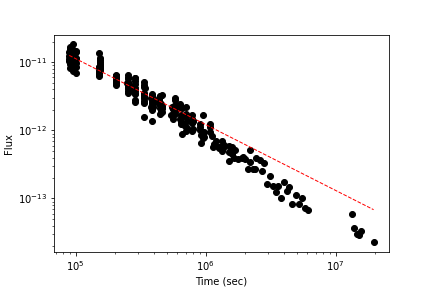
\includegraphics{analysis/Long_GRBs/130702A/130702A_fit.png}[scale=0.2]
\section{Validity and reliability of data }
 As mentioned in section 3.3, examine the data then to get the information about object under taken , we already decided to follow both quantitative and qualitative approaches , standared models and tools were  proposed  to use in analyzing the data collected so as to achieve the desired  objectives and give answers  for the  statements of problems mentioned in section 1.5. This might be  keep the validity and reliability of our work.
\section{Data processing and analyzing} 
\subsection{Data processing }
As mentioned in section 3.3 above , sample of  twenty  gamma -ray bursts ( long and short ) were collected to  analyze. To extract relevant information and conclusions  that support for final  judgment  data of the sampled  GRBs  were cleaned by avoiding  duplicated  and incorrect data , missing values and outliers.  
\subsection{Data analyzing}
Using python 3 program language , graphical relation between X-ray  flux (F)  and time (t) has been shown for the sampled  data. Hereafter considering high latitude radiation and the flux decay closure relations, we made a numerical determinations
of temporal and spectral indices of the afterglow decay for early steep decay and temporal index for the rest phases.\\
A) analysis of short GRBs with 1  and  2 light curve breaks:\\
I use simple power law \\
B) analysis of long GRBs with 1  and  2 light curve breaks:\\
C)analysis of short GRBs with 3 light curve breaks :\\
D)analysis of long GRBs with 3 light curve breaks:\\